\documentclass[12pt,a4paper]{article}
\usepackage[a4paper]{geometry}
\usepackage{fullpage}
\usepackage{url}
\usepackage[backend=bibtex]{biblatex}
\usepackage{caption}
\usepackage[utf8]{inputenc}
\usepackage{enumerate}
\usepackage{tabularx}
\usepackage{graphicx}
\usepackage{float}
\usepackage{color}
\usepackage{amssymb,amsmath,wasysym}
\usepackage{enumitem}

\addbibresource{bib1.bib}

\begin{document}

\title{Computational Intelligence, SS2017, Assigment 6}

\author{%
\name{Lucas Reeh}
\email{lreeh@student.tugraz.at}
}
\date{\today}

\begin{titlepage}
   \begin{center}
     \begin{huge}
		   %% Update assignment number here
           \textbf{Assignment 6}
     \end{huge}
   \end{center}

   \begin{center}
     \begin{large}
           Computational Intelligence, SS2017
     \end{large}
   \end{center}

   \begin{center}
 \begin{tabularx}{\textwidth}{|>{\hsize=.33\hsize}X|>{\hsize=.33\hsize}X|>{\hsize=.33\hsize}X|} 

           \hline
           \multicolumn{3}{|c|}{\textbf{Team Members}} \\
           \hline
           Last name & First name & Matriculation Number \\
           \hline
           Reeh & Lucas & 00630182 \\
           \hline

     \end{tabularx}
   \end{center}
\end{titlepage}

\tableofcontents
\listoffigures

\newpage

\section{Expectation Maximization Algorithm}

\begin{figure}[H]
  \centering
  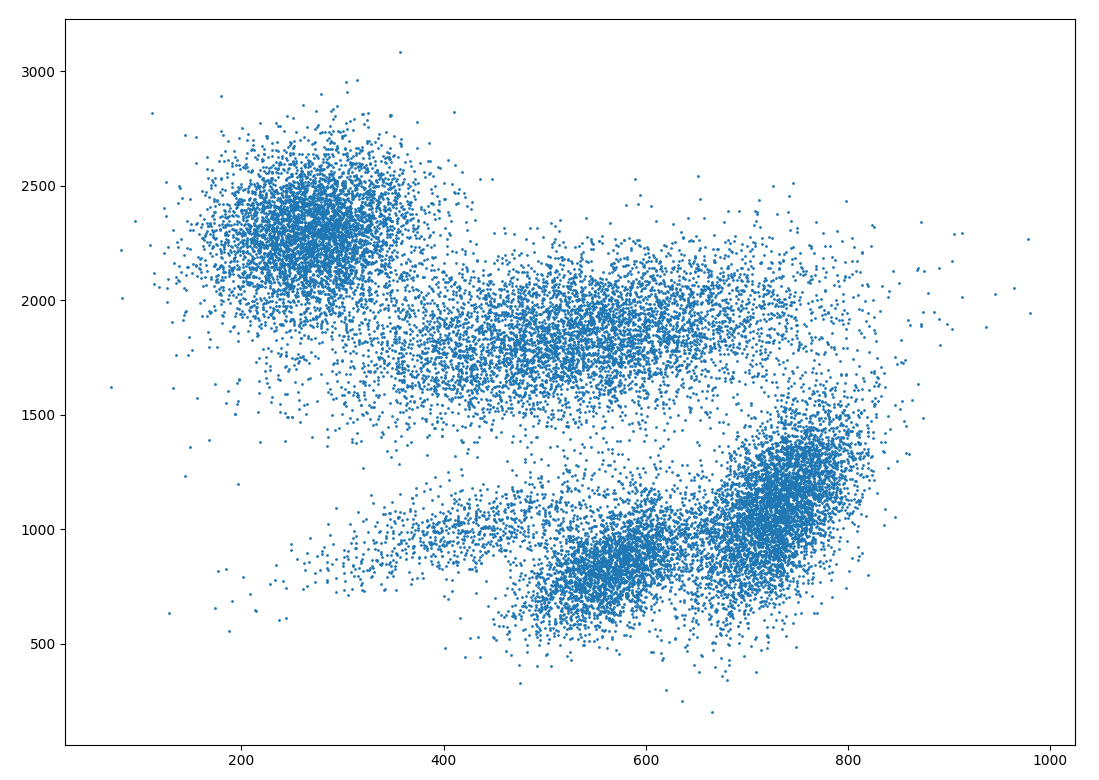
\includegraphics[width=0.8\textwidth]{figures/1_0.png}
	\caption{Training Data}
	\label{1_0}
\end{figure}

\setcounter{enumi}{2}
\begin{enumerate}[start=2,label*={\arabic*.}]
  % 1
  % 2
  \item Correct number of components $M = 5$ (fixed random seed)

\end{enumerate}

\newpage
\section{ Samples from a Gaussian Mixture Model}

\newpage
\printbibliography

\end{document}